
\chapter{Getting Started with \emph{Ravel}}

\section{System requirements}

\emph{Ravel} is a proprietary program for data analysis which
currently only runs on Windows (version 8 and later). It consists of a
plugin for the \emph{Ravel application}, also known as \emph{Minsky},
which is an open source program available for Windows, Mac OS X,and
various Linux distributions. After obtaining Minsky (from the
\htmladdnormallinkfoot{Patreon Store}{https://www.patreon.com/hpcoder}),
  you will need to select ``Upgrade'' from the File menu to install
  the latest version of the Ravel plugin.

Some components of the interface are specific to \emph{Minsky}. This
``Getting Started'' guide focuses on the components used by
\emph{Ravel}. For a getting started guide to see \htmlref{\emph{Minsky}}{Introduction-Minsky}.

\section{Getting help}

Press the F1 key, or select ``help'' from the context menu. Help
is context-sensitive. If you press F1 while the mouse is hovering
over a widget--for example, the addition block--then the help window
will appear with instructions on how to add elements together.

\section{The Ravel Interface}

There are 5 main components to the \emph{Ravel} interface:
\begin{enumerate}
\item The Menus;
\item The Operations controls;
\item The Tabs: The Design Canvas and its documentation companions Equations,
Summary, Phillips Diagram, and Publication(s);
\item The Design icons (sometimes called Operators or Widgets in this help
file); and
\item The Design Canvas.
\end{enumerate}
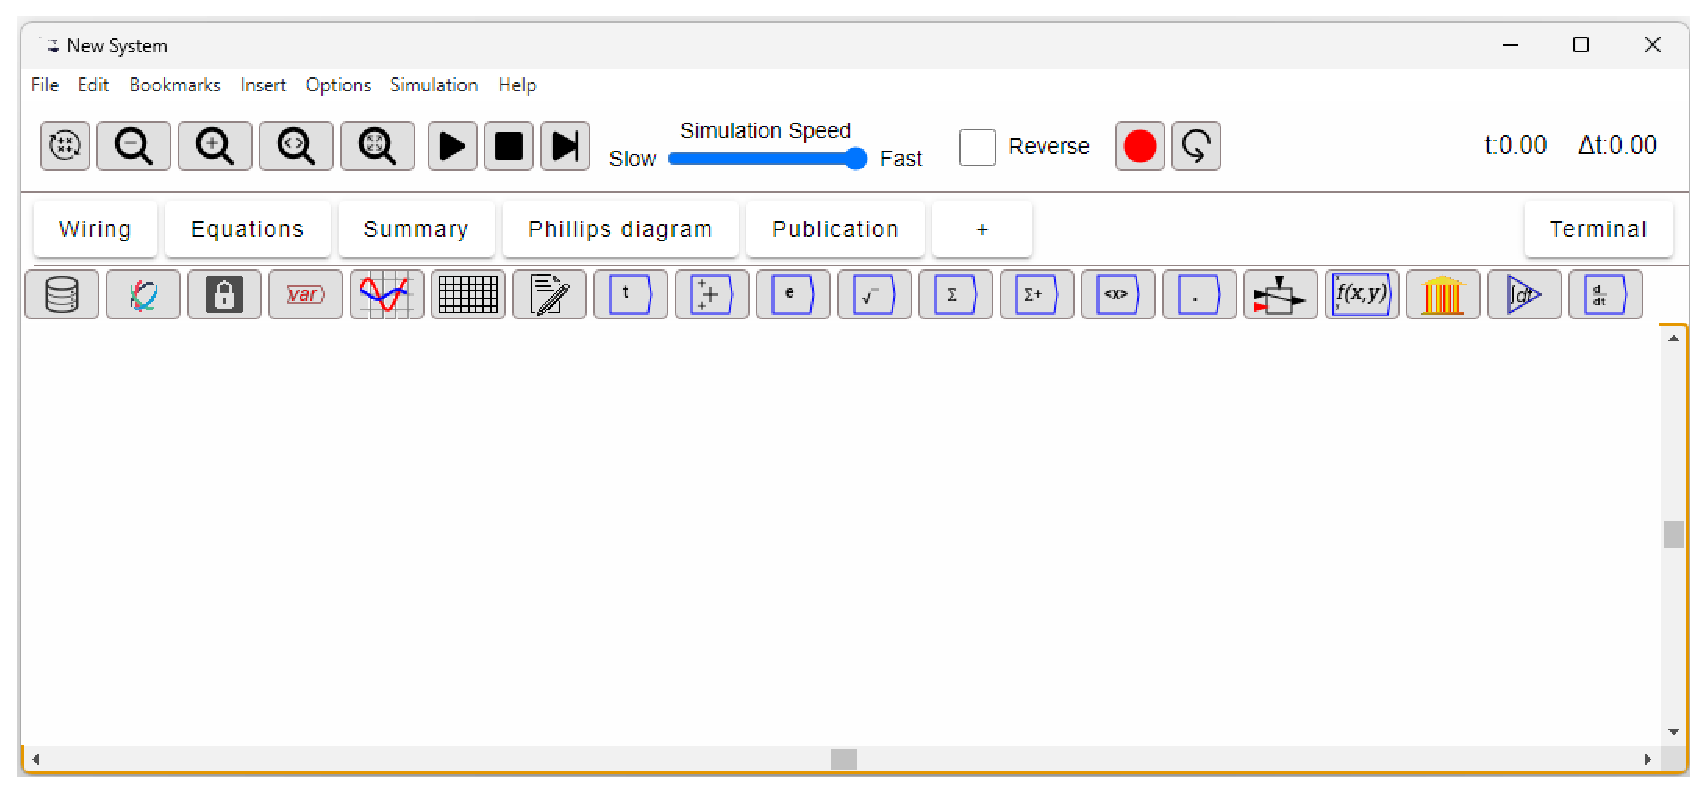
\includegraphics[width=15cm]{images/Interface}

\subsection{Menus}

\label{Menu}

The menu controls the basic functions of saving and loading files,
default settings for the program, etc. These may alter as the program
develops; the current menu items (as of June 2024) are:

\begin{tabular}{lllllll}
File  & Edit  & Bookmarks  & Insert  & Options  & Simulation  & Help \tabularnewline
\end{tabular}

\subsubsection{File}

\label{File}
\begin{description}
\item [{About}] Tells you the version of \emph{Ravel} and/or \emph{Minsky}
  that you are using.
\item[Upgrade] Will upgrade you to the latest release of Minsky, and
  if subscribed for Ravel updates, also install the latest version of Ravel.
\item [{New System}] Clear the design canvas. If you have made changes
and haven't saved them, you will be prompted to save before the canvas
is cleared.
\item [{Open}] Open an existing \emph{Ravel} or \emph{Minsky} file. \emph{Ravel}
files have the suffix of ``rvl'', \emph{Minsky} files have the suffix
of ``mky''. Technically they are identical, with the only difference
being that RVL files contain a Ravel while MKY files do not.
\item [{Recent Files}] \label{recentfiles} Provides a shortcut to some
of your previously opened \emph{Ravel} (or \emph{Minsky}) files. \emph{Ravel}
files have the suffix RVL and \emph{Minsky }files have the suffix
MKY.
\item [{Library}] Opens a web-based repository of models for the \emph{Minsky}
simulation system.
\item [{Save}] Save the current file.
\item [{Save As}] Save the current file under a new name.
\item [{Insert File as Group}] Insert a \emph{Ravel/Minsky} file directly
into the current model as a \htmlref{Group}{Group}.
\item [{Dimensional Analysis}] As processing networks
get more complex, it is useful to attach units to the
data. Dimensional analysis then checks that the mathematical
operations are allowable---rejecting, for example, adding feet to
metres.
\item [{Export Canvas as}] Export the current canvas in svg, pdf, eps,
tex, or m format for use by other programs. The current canvas (which
varies depending on which Tab you have open) can be exported in a
number of different formats:
\begin{description}
\item[SVG] This is a ``vector graphics'' format which can be inserted into
word processing (such as Word or OpenOffice) or presentation (Powerpoint
etc.) documents. 
\item[PDF] This saves the currently displayed canvas as an Adobe Acrobat
file .
\item[EMF] This saves the canvas in an enhanced form of the WMF (Windows
Metafile) vector graphics standard, for use in documentation programs
like Powerpoint and Word. This is only available in the Windows
version of Minsky.
\item[Postscript] This saves the canvas in an encapsulated form of PDF.
\item[Portable Network Graphics] This saves the canvas in a bitmap file (PNG)
for use in paint and photo programs, etc. 
\item [LaTeX] This exports the equations in a model in a mathematical formatting
language called \LaTeX. This file can be imported into mathematics
programs like MathType to document the mathematical logic in your
model. If you are a \LaTeX{} user yourself, you can load this directly
into your preferred \LaTeX{} editor.

If your LaTeX implemention doesn't support breqn style, untick the \htmlref{wrap
long equations option}{wrap-equations}, which can be found in the
preferences panel under the options menu. 
\item [Matlab] This exports the model as an ``.m file'' for importing into
the algebraic program Matlab. This enables the analysis and simulation
of your model in a MatLab compatible system, such as Matlab itself
\url{https://en.wikipedia.org/wiki/MATLAB} or Octave \url{http://www.gnu.org/software/octave}.
\end{description}
\item [{Log simulation}] This \emph{Minsky}-specific command outputs the
results of simulated variables into a CSV data file for later use
in other programs.
\item [{Recording}] This \emph{Minsky}-specific command records the states
of a model as it is being built for later replay.
\item [{Replay recording}] This \emph{Minsky}-specific command replays
a recording of model states.
\item [{Quit}] Exit the program. \emph{Ravel} will check to see whether
you have saved your changes. If you have, the program will close;
if not, you will get a reminder to save your changes.
\item [{Debugging use}] Items under the line are intended for developer
use, and will not be documented here. All programs have bugs! If you
experience one, please report it via the \htmladdnormallink{SourceForge ticket system}{https://sourceforge.net/p/minsky/tickets/}.
\item [{Redraw}] Redraw may be useful if the screen gets messed up because
of a display bug. For example, a bug could cause items on the canvas
to be scaled differently. Redraw could overcome this problem without
requiring you to exit the program.
\end{description}

\subsubsection{Edit}

\label{Edit}
\begin{description}
\item[Undo and Redo] \label{edit:undo}  allow you to step back and forward
in your editing history. If you undo a few edits, and then change
the model at that point, the undo history is then reset to commence
with your new edit. \emph{Ravel} supports the standard Windows shortcuts
of control-Z for undo and control-Y for redo.
\item[Cut/copy/paste] \label{edit:copy}  Selecting, or lassoing a region
of the canvas will select a group of icons, which will be shaded to
indicate the selected items. Wires joining two selected items will
also be selected. Note that, compatible with X-windows, selecting
automatically performs a copy, so the copy operation is strictly redundant,
but provided for users familiar with systems where an explicit copy
request is required. Cut deletes the selected items. Paste will paste
the items in the clipboard as a \htmlref{Group}{Group} into the current
model. \emph{Ravel} supports the Windows-standard shortcut keys of
control-C for copy, control-X for cut (which deletes the entity at
the current location and creates a copy for pasting elsewhere) and
control-V for paste.
\item[Group selection] \label{edit:group} Create a \htmlref{Group}{Group} using
the contents of the selection. Groups allow you to organise more complicated
systems components into aggregated modules that make the overall system
more comprehensible. In \emph{Ravel}, groups can be used to, for example,
collect all the file importing operations into a Group, thus removing
the details of these operations from the top level view. This reduces
the complexity of a canvas, which can make it easier for both the
developer and viewers to focus on the analysis that the document is
actually doing.
\item[Dimensions] \label{edit: Dimensions} This invokes the Dimensions dialog box,
which lists the Dimensions (Ravel axes) in a document, their type
(string, time, value), and their units or formatting.
\item[Remove Units] removes all units from the system, effectively
  disably dimensional analysis.
\item[Auto Layout and Random Layout] change the layout of your
  model. These commands are still under development, so are currently
  not recommended unless you have all items sitting on top of each
  other. If you do accidently select one of these commands and mess up
  your model layout, simply press ``undo''.
\end{description}

\subsubsection{Bookmarks}

\label{Bookmarks} Bookmarks store the location and scaling of a model
for future reference. This is an alternative to grouping as a means
to organize a model. To create a bookmark, either:
\begin{itemize}
\item Move the canvas and zoom it to the level at which all the items you
wish to bookmark are visible. Then click on the Bookmark menu and
choose ``Bookmark this position''. Give the Bookmark a name and it
will be added to this menu. To move to that location in the model,
click on this Bookmark name. Bookmarks can be deleted using the ``Delete
bookmark'' sub-menu. Or
\item Insert a text box at the upper left location and click the Bookmark?
checkbox. The Short Description of the textbox is used as the name
for the Bookmark. Both the upper left location shown on the canvas
and the zoom level in operation at the time of the Bookmark's creation
are saved, and restored when that Bookmark is selected from the Bookmarks
menu.
\end{itemize}

\subsubsection{Insert}

\label{Insert}

This menu contains all the mathematical \htmlref{operator blocks}{Operations}
used in \emph{Ravel}, and enables you to place those operators on
the Canvas. You can get the same effect by clicking on the Design
Icons. A Ravel can be inserted from this menu, as can Plots, Sheets
and \emph{Minsky}-specific tools like \htmlref{Godley Tables}{Godley-Tables}.

\subsubsection{Options}

\label{Options}

The options menu allows you to customise aspects of \emph{Ravel} and
\emph{Minsky}. At the moment most options pertain to \emph{Minsky}
rather than \emph{Ravel}, but this will change as \emph{Ravel} increases
in complexity. In this section of the manual we ignore options pertaining
only to \emph{Minsky}; these are covered in \htmlref{\emph{Introduction
  to Minsky}}{Introduction-Minsky}
\begin{description}
\item [{Preferences}] %
\mbox{%
%
}
\begin{itemize}
\item Number of recent files to display --- this determines how many previously
edited files are displayed on the \htmlref{Recent files}{recentfiles}
menu. 
\item \label{wrap-equations} Wrap long equations in \LaTeX{} export. If ticked,
\emph{Ravel} \& \emph{Minsky} will use the \LaTeX{} ``breqn'' package
to produce nicer looking automatically line-wrapped formulae. Because
not all \LaTeX{} implementations are guaranteed to support breqn, untick
this option if you encounter problems. 
\item \label{font} select a font for variable names, parameter names, etc. 
\end{itemize}
\item [{Background colour}] --- select a colour for the wiring canvas.
The default is white.
\end{description}

\subsubsection{Simulation}

These commands are specific to \emph{Minsky} and control how a model
is simulated. They are covered in the \htmlref{\emph{Minsky} component of this
manual}{Introduction-Minsky}. 

\subsubsection{Help}

\label{Help}

Provides an in-program link to this manual. Note that pressing F1
will also launch help windows in a context-sensitive way. That is,
it will open the relevant help section for whatever object the mouse
is currently hovering over. Similarly, each item on the canvas has
a help menu item in the context menu relevant for that item.

\subsection{The Operation Controls}

These controls cause \emph{Ravel} to recalculate a model; zoom in
and out on the canvas; run and control the speed and direction of
a \emph{Minsky} simulation model; and record and replay the process
of building a model.

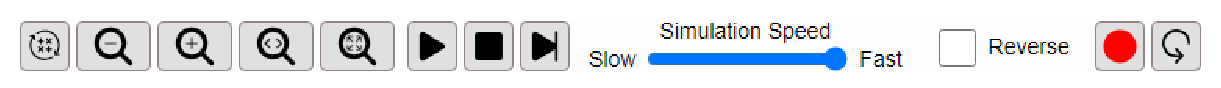
\includegraphics[width=15cm]{images/OperationsControls}

\subsubsection{Recalculate button}


\includegraphics{images/Recalc}

The recalculate button computes the values of all variables in a model.
\emph{Ravel} will periodically recalculate a document, but this is
a useful option if you wish to immediately see the results of a calculation.

\subsubsection{Zoom buttons}

\label{ZoomButtons}


\includegraphics{images/ZoomControls}

The Zoom buttons \buttonIcon{zoomIn.eps} and \buttonIcon{zoomOut.eps}
zoom in and out on the wiring canvas. The same functionality is
accessed via the mouse scroll wheel. The reset zoom button
\buttonIcon{zoomOrig.eps} resets the zoom level to 1, and also
recentres the canvas. The Zoom to Fit button
\buttonIcon{zoomToFit.eps} zooms the model so that it just fits in the
current canvas window.

\subsubsection{Run Buttons}

These commands are specific to \emph{Minsky} and are covered in the
\emph{Minsky} component of this manual.

\subsubsection{Speed slider, time direction and model recording}

These commands are specific to \emph{Minsky} and are covered in detail
in the \emph{Minsky} component of this manual.

The speed slider controls the rate at which a model is simulated.
The ``Reverse'' checkbox causes the simulation to run backwards
rather than forwards in time. 

The Record and Replay buttons respectively record the process of creating
a model, and replay that process. 

\subsubsection{Simulation time}

In the right hand top corner is a textual display of the current simulation
time $t$, and the current (adaptive) difference between iterations
$\Delta t$. This information is specific to a \emph{Minsky} simulation
model.

\subsection{Tabs}

\subsubsection{Wiring Tab}

\label{tabs:wiring}

The Wiring Tab is where a \emph{Ravel} document is designed: see
\htmlref{\emph{Design Canvas}}{DesignCanvas}
for its components.

\subsubsection{Equations tab}

\label{tabs:Equations}

This displays the mathematical representation of the document, which
enables you to see the complete mathematical logic in a document.
You can also export a full \LaTeX{} rendition of the document (from the
File:Export Canvas command) to a \htmlref{\LaTeX-capable editor}{Export}.

\subsubsection{Summary Tab}

\label{tabs:Summary}

This tab provides a summary table of all variables in the system,
in a heirarchical fashion. Each variable is fully documented including
its name, definition, dimensions (for tensor-valued variables), units
and current value.

For example, this is a \emph{Ravel} file modelling the economics textbook
concept of a profit-maximizing firm.

\noindent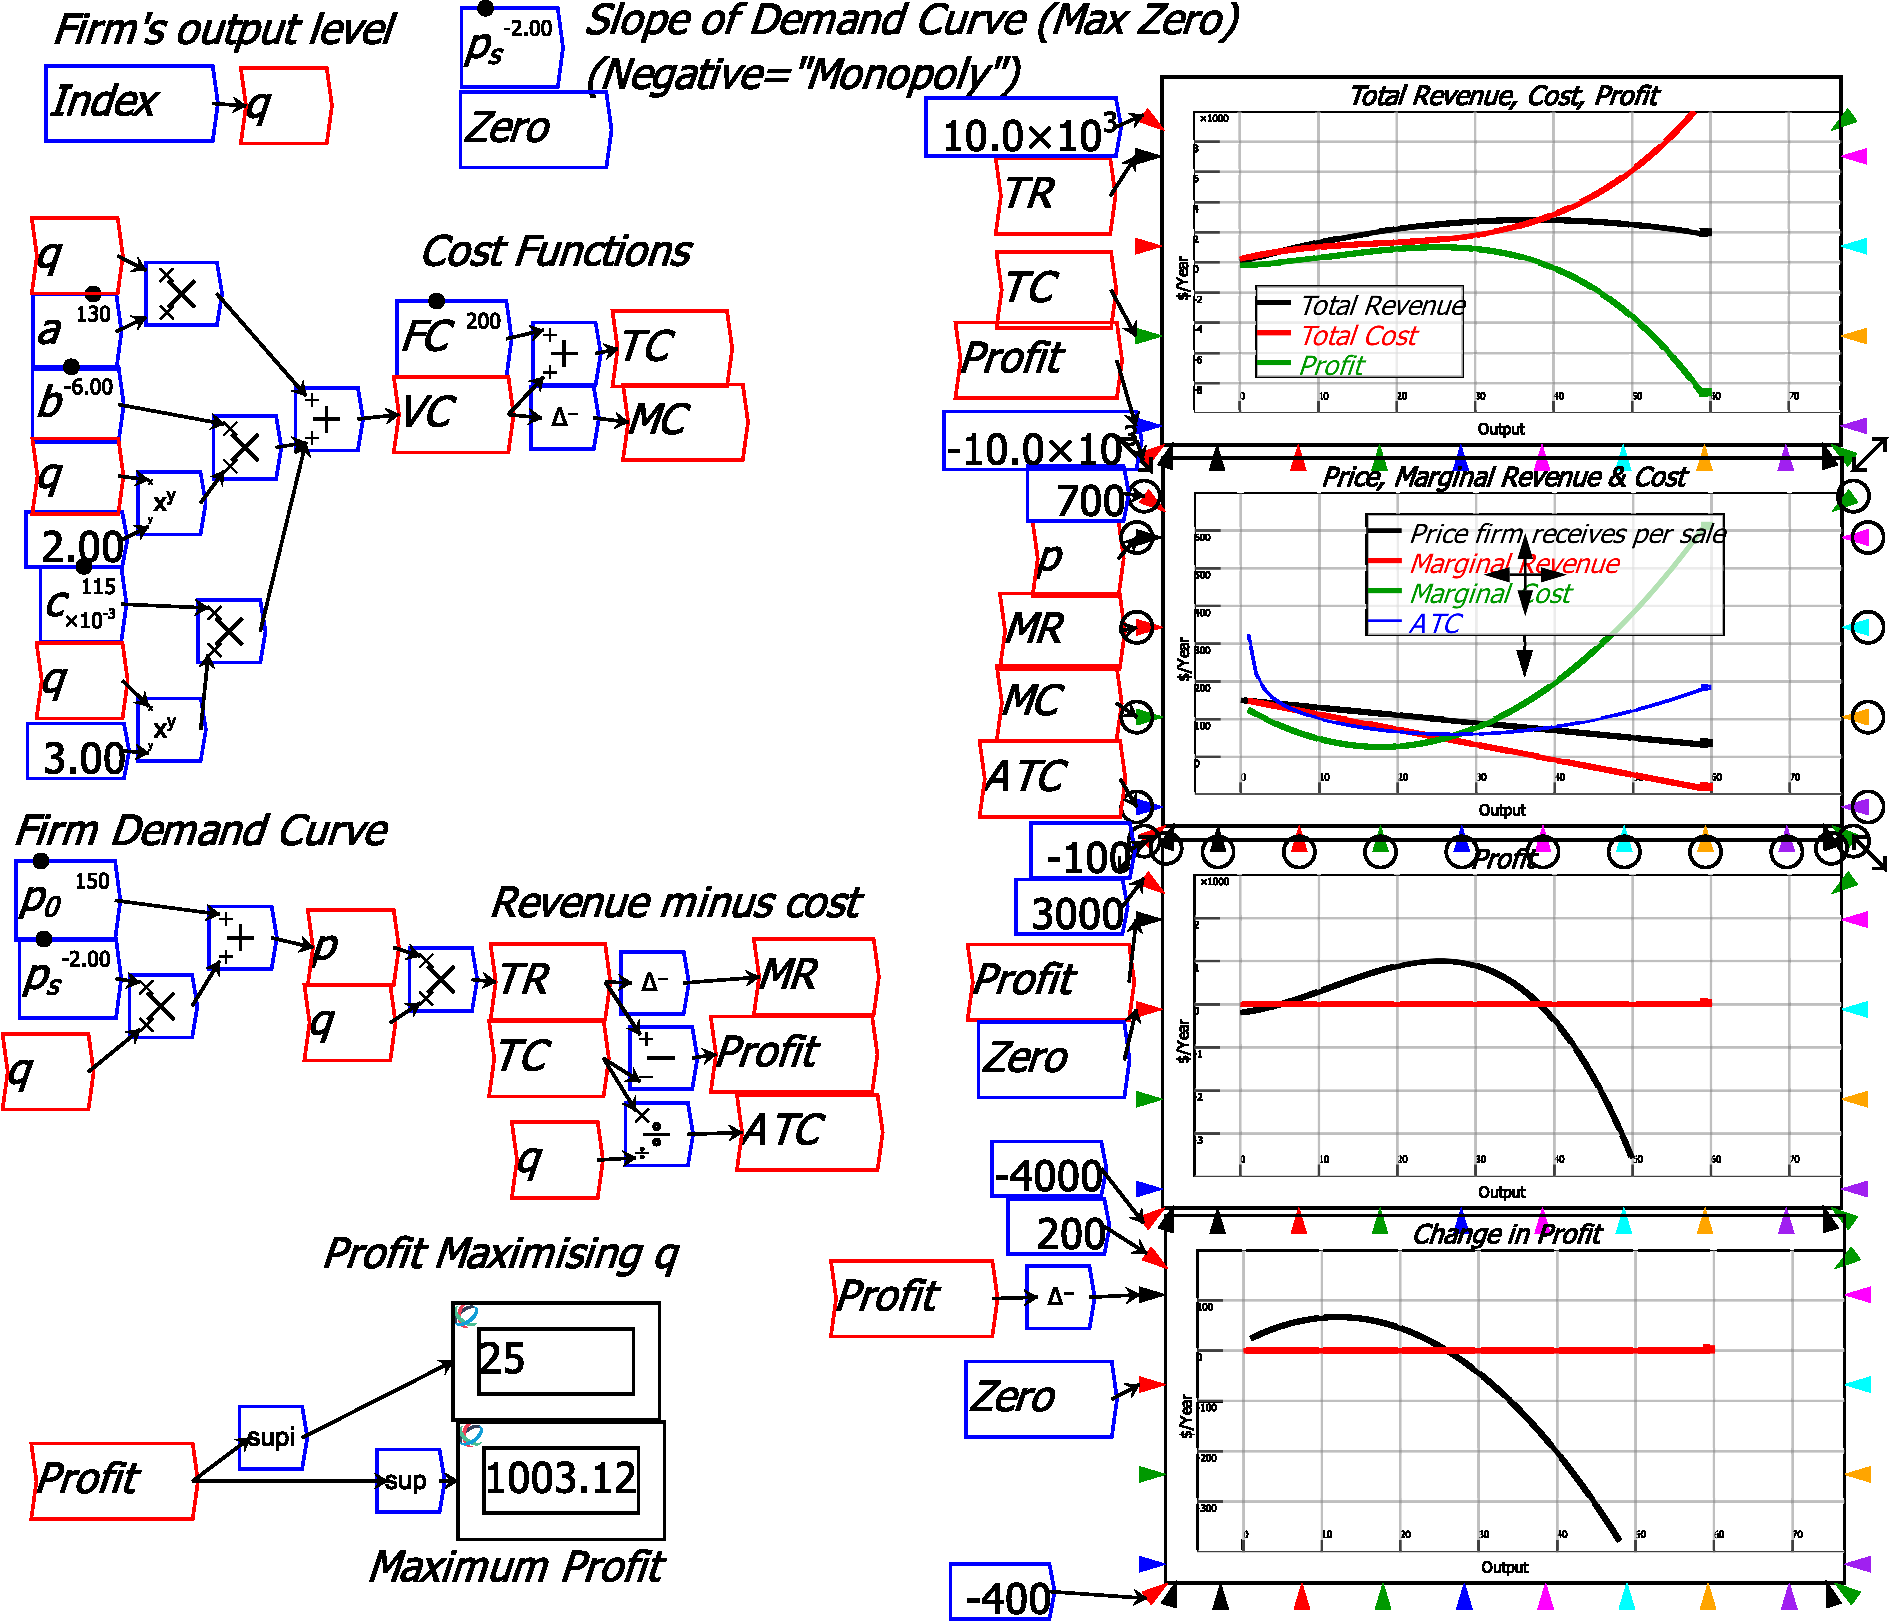
\includegraphics[width=\textwidth]{images/NeoclassicalModelOfFirm}

The next figure shows an extract from the summary tab documentation
for this model.

\noindent\includegraphics[width=\textwidth]{images/SummaryTabScreenshot}

This document imports data from the Bank of International Assessments,
separates the data into a number of variables, and uses data on debt
in domestic currency and debt as a percentage of GDP to derive GDP
in domestic currency data.

\noindent\includegraphics[width=\textwidth]{images/DebtCalcGDPexample}

This is the Summary Tab for that model, showing the variable names,
their mathematical definitions, their dimensions, and any initial
values assigned to them.

\noindent\includegraphics[width=\textwidth]{images/DebtCalcGDPexampleSummaryTab}

Most of these fields are editable. Changing a variable's name will
do a \emph{replace all instances} operation to update all variables
of the same name. Changing a variable's definition will replace the
wiring graph leading into the variable by a \htmlref{user defined function}
{Operation:userFunction} containing your edited string. At some
future point, functionality will be added to convert a user defined
function into a wiring graph.

\subsubsection{Phillips diagram tab}

\label{tabs:Phillips}

This is a \emph{Minsky}-specific feature which is covered in the \emph{Minsky
}sections of this manual.

\subsubsection{Publication tab}

Publication tabs allow the creation of dashboards to emphasise certain
aspects of your data analysis in \emph{Ravel }(or simulation in \emph{Minsky}).
For example, you may wish to provide different reports on the same
data for the Accounting and Marketing sections of your company.

Multiple publication tabs can be created by clicking the `+' tab.
See \htmlref{\emph{Publication tabs}}{tabs:Publication} for full details.

\subsection{Design Canvas}

\label{DesignCanvas}

The Design Canvas is where you develop your model. It has two components:
\begin{itemize}
\item The \htmlref{Operations}{Operations} icons, which give access to all of
\emph{Ravel}'s objects and mathematical operations; and
\item The canvas itself, which is a space on which these objects and operations
can be placed and connected by wires to perform data analysis, modelling,
and displaying of results in Sheets and Plots.
\end{itemize}
A model consists of a number of blocks---imported data in parameters,
Ravels, user-defined parameters, variables, constants, mathematical
operators and the display elements (plots and sheets)---connected
by wires.

The canvas is \emph{zoomable}, either via the zoom buttons on the
toolbar, or via the mouse scroll wheel. It is also \emph{pannable},
either via the scroll bars on the right and bottom, or by holding
the shift key and left mouse button together. 

\noindent\includegraphics[width=\textwidth]{images/DesignCanvas}

The canvas is effectively unlimited, however the scroll bars treat
the canvas as $10000\time10000$ pixels in size.

\subsubsection{Wires}

The wires in a model connect blocks together to define equations.
For details see \htmlref{\emph{Wires}}{Wires}

\subsubsection{Design Icons}

\noindent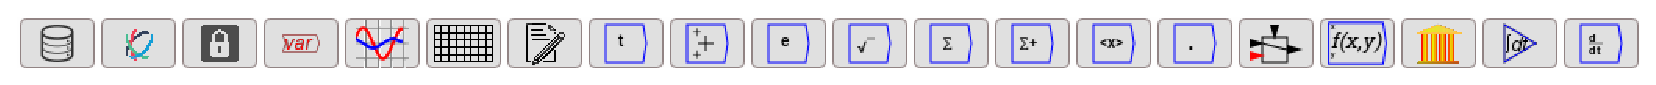
\includegraphics[width=\textwidth]{images/DesignIcons}

These are the ``nuts and bolts'' of data analysis using \emph{Ravel}.
There are many icons, and more will be added over time as we extend
\emph{Ravel}'s capabilities.

The critical icons for \emph{Ravel} are the first four: Import Data
\buttonIcon{importData.eps}; insert a Ravel \buttonIcon{RavelIcon};
attach a selected slice of the Ravel to a Lock; and attach that lock
to a variable for further analysis.
\begin{description}
\item [{Import data}] \buttonIcon{importData.eps} Opens an import CSV
file dialog, which allows a CSV file to be loaded into a parameter
in Ravel (the default name of the parameter is the name of the file
being imported). See \htmlref{\emph{Importing CSV files}}{CSV import} for
full details. After a data file is imported, the next step is to attach
it to a Ravel.
\item [{Ravel}] \buttonIcon{RavelIcon} This places a Ravel on the
wiring canvas. The first time this is done in a document, the Ravel
is displayed full-size in Edit mode, and a sample set of dimensions
are displayed. Subsequent Ravels are displayed in icon mode. For full
details on using a Ravel see \htmlref{\emph{Ravel GUI}}{Ravel-GUI Object}.
\item [{Lock}] \buttonIcon{Lock} Lock widgets are used with
Ravels. A lock keeps a record of the current state of a Ravel: the
items selected on its axes, the effect of calipers in selecting data
ranges, and so on. You can then manipulate the Ravel without changing
the output from the Lock, which can be assigned to a variable for
further use. You can also impose the state of a Lock on its associated
Ravel---this is useful if you wish to fine tune the output from the
Lock. See \htmlref{\emph{Lock}}{Lock} for full details. The output of a Lock will
change whenever the attached data file changes.
\item [{Variable}] \buttonIcon{var.eps} \label{Variable}
This is a pop-up menu, which gives access to the form that creates
variables, constants and parameters, and access to the Browser, which
is a window that lists all the variables and parameters in a model,
and enables them to be placed on the wiring canvas.

Variables are entities whose value changes as a function of time and
its relationship with other entities in your model. Click on it and
a variable definition window will appear:
\item [{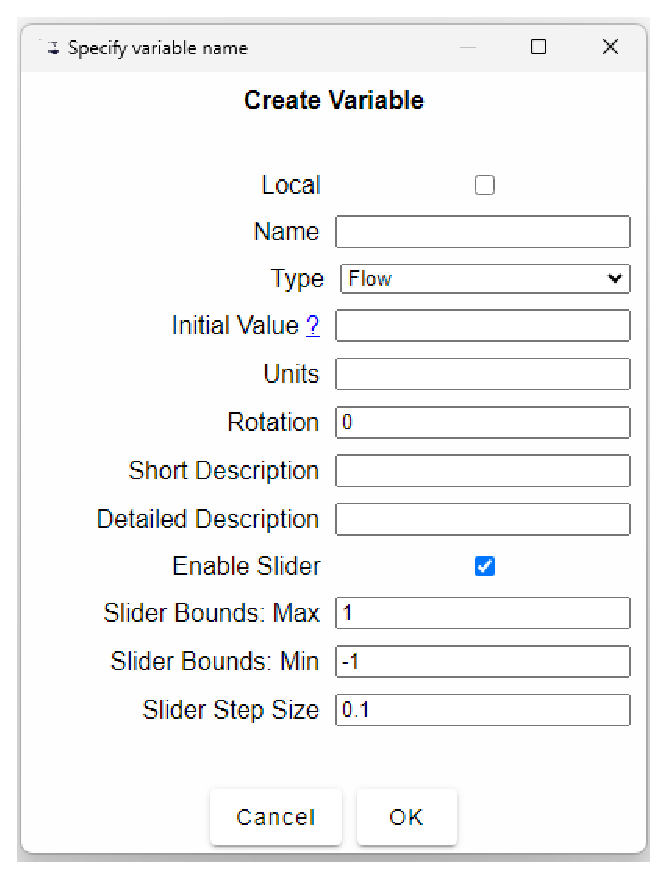
\includegraphics[width=10cm]{images/VariableDefinitionForm}}]~
\end{description}
See \htmlref{Variables}{Variables} for full details on using this form.
\begin{description}
\item [{Plot widget}] \buttonIcon{plot.eps} Add Plots to the canvas.
See \htmlref{Plot widget}{PlotWidget} for full details.
\item [{Sheet widget}] \buttonIcon{sheet.eps} Add a Sheet---for the
display of numerical data to the canvas. See \htmlref{Sheet}{Sheet} for full
details.
\item [{Notes}] Add textual annotations to a document. See \htmlref{Notes}{Notes}
for full details.
\item [{Time}] \buttonIcon{time.eps} embeds a reference to the simulation
time on the Canvas. This is a \emph{Minsky}-specific feature.
\item [{Fundamental}] constants. These include e, $\pi$, 0, 1 and the
percentage operator. See \htmlref{Special constants}{Special-constants} for full details.
\item [{Binary operations}] \buttonIcon{BinaryButton.png}. These execute
the stated binary mathematical operations: operations that require
two (or more) inputs. Where appropriate, each input port to a binary
operator can take multiple wires---so that to add five numbers together,
for example, you can wire 1 input to one port on the Add block, and
the other four to the other port. The same applies to the subtract,
multiply, and divide blocks. See \htmlref{Binary Operations}{Binary-Operations} for full
details.
\item [{Unary functions}] \buttonIcon{sqrt.eps} These are a fairly standard
complement of mathematical functions which take only one input--though
this input can have multiple dimensions. See \htmlref{Unary functions}{Functions/Unary-Operators}
for details.
\item [{Reduction operations}] \buttonIcon{sum.eps} This menu contains
operations such as sum, product, any, all, etc., that reduce a vector
to a scalar, or reduce the rank of a tensor. See \htmlref{Tensor operations}{Operations: Reduction}
for details.
\item [{Scans}] \buttonIcon{runningSum.eps} This menu contains operations
running sum, running product, and the difference operators. See \htmlref{Tensor operations}{Operations: Reduction}
for details.
\item [{Miscellaneous tensor operations}] \buttonIcon{outerProduct.eps}
Any other tensor function not covered elsewhere.
\item [{Switch}] \buttonIcon{switchIcon.eps} Add \htmlref{a piecewise-defined
function block}{SwitchIcon} to the canvas. See \htmlref{Switch}{SwitchIcon}
for details.
\item [{User defined function}] \buttonIcon{userFunction.eps} You can
define your own function using an algebraic expression, such as \verb+exp(-x^2+y)+.
See \htmlref{User defined functions}{Operation:userFunction}for details.
\item [{Godley Table}] \buttonIcon{NewItem29.eps}. \label{GodleyTable}
This is the fundamental element of \emph{Minsky} that is not found
(yet) in any other system dynamics program. It is covered in the \htmlref{\emph{Minsky}
chapter of this manual}{Introduction-Minsky}.
\item [{Integration}] \buttonIcon{int.eps}. This inserts a variable whose
value depends on the integral of other variables in the system. It
is discussed further in the \emph{Minsky} section of the manual.
\item [{Derivative Operator}] \buttonIcon{differentiate.eps} This operator
symbolically differentiates its input. It is a component of \emph{Minsky}
which is explained in the \emph{Minsky} section of this manual.
\end{description}

\section{Working with \emph{Ravel}}

Data analysis is performed in Ravel by connecting components using
\htmlref{wires}{Wires} on the Wiring canvas.

\subsection{Components in \emph{Ravel}}

There are several types of components:
\begin{enumerate}
\item Parameters, which either load in data from an external CSV file, store
values typed in by the user, or create arrays of numbers using simple
formulas entered into the \emph{Initial Value} field;
\item Ravels, which take data from a parameter and create a multi-dimensional
graphical rendition of the data; 
\item Mathematical operators such as plus (+), minus (-), etc. These are
all aware of the dimensions of your data, so they act on arrays of
data, rather than single cells as with spreadsheet formulas; 
\item Constants, which are given a value by the user;
\item Variables whose values are calculated by the program and depend on
the values of constants, parameters and other variables, and the formulas
applied to them;
\item Text strings and paragraphs, which can be used to document a model;
and
\item Groups, which allow components to be grouped into modules that can
be used to construct more complex models. 
\end{enumerate}

\subsection{Inserting a component}

There are five ways to insert a component onto the Canvas: 
\begin{enumerate}
\item Click on the desired Icon on the Icon Palette, drag the block onto
the Canvas and click the mouse where you want to insert it
\begin{center}
\fwhtmladdimg{NewItem18.png} 
\par\end{center}
\item Choose Insert from the menu and select the desired block there

%begin{latexonly}

\begin{center}
\resizebox{!}{0.6\textheight}{ %end{latexonly}
 \htmladdimg{NewItem159.png} %begin{latexonly}
 } %end{latexonly}
 
\par\end{center}

\newpage{}
\item Right-click on an existing block and choose copy. Then place the copy
where you want it on the palette.
\begin{center}
\htmladdimg{NewItem161.png} 
\par\end{center}
\item Variables can be inserted by typing the variable name on the canvas,
and constants can be entered simply by typing the number on the canvas.
Similarly, operations can be inserted by typing the operator name
(eg \verb+sin+, or \verb+*+). Notes can be inserted by starting
the note with a \verb+#+ character.
\item Variables can also be picked from the \htmlref{Variable Browser}{VariableBrowser}
and placed on the canvas. 
\end{enumerate}

\subsection{Creating an equation}

Equations are entered in \emph{Ravel} graphically. Mathematical operations
like addition, multiplication and subtraction are performed by wiring
the inputs up to the relevant mathematical block. The output of the
block is then the result of the equation.

For example, a simple equation like 
\[
ProfitMargin=(Price-Cost)/Cost
\]
is performed in \emph{Ravel} by :
\begin{center}
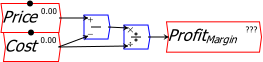
\includegraphics[width=10cm]{images/ProfitMarginEquation} 
\par\end{center}

If you click on the Equation or Summary Tab, you will see this flowchart
rendered as an equation:

\[
Profit_{Margin}=\frac{Price-Cost}{Cost}
\]

If the variables Price and Cost were multi-dimensional---if, for
example, they stored price and cost data for different \emph{products}
at different \emph{stores} at different \emph{dates}---then this
one formula would calculate profit margins \emph{by product by store
by date}.

\subsection{Wiring components together}

A model is constructed by wiring one component to another in a way
that defines an equation. Wires are drawn from the output port of
one block to the input port of another. Ports are circles on the blocks
to which wires can be attached, which can be seen when hovering the
pointer over the block. Variables have an input and an output port;
constants and parameters only have an output port. A mathematical
operator has as many input ports as are needed to define the operation.
Some operators can be ``overloaded''---more than one input can
be attached to an input port. Thus you can add more than two variables
using the \buttonIcon{add}block, simply by wiring more
than one variable to each input port. The same applies to the subtraction
block \buttonIcon{minus}, division \buttonIcon{Divide},
minimum \buttonIcon{min} and maximum \buttonIcon{max}
blocks.
